% !TeX encoding = UTF-8
% !TeX spellcheck = en_US
% !TeX root = report1.tex


\section{Monte Carlo Integration}

First, we explored different methods and compared the results obtained
in order to gain a better insight on how to create a better general integrator. Each method differs in how
the points in the domain are chosen to evaluate the integral.
The integration schemes \cite{MCmethods} used are:
\begin{enumerate}
  \item Uniform Static - The entire domain is divided by a uniform mesh were each point is taken in a coordinate is the grid.
  \item Adaptive - The domain is divided uniformly in square boxes, and for each box a mesh grid is created
  specified by a density value which determines the total number of points inside that box. The density parameter
  is obtained by performing successive iterations, on which the density of each sub-box is set by the total value of the integral inside
  the box.
  \item Stratified Static - The entire domain is divided in a uniform mesh, where for each quadrant of the mesh
  a single point is chosen randomly inside.
  \item Adaptive Stratified - Basically a combination of both methods adaptive and stratified.
\end{enumerate}

To compare each we used a test function on which we evaluated the different integrals.
The test function consisted on a donut shaped  in a 2-dimensional domain. The resulting
sample points for each method are shown in fig. \ref{} and the table below shows the error
obtained in each case.

\begin{figure*}
  \begin{center}
  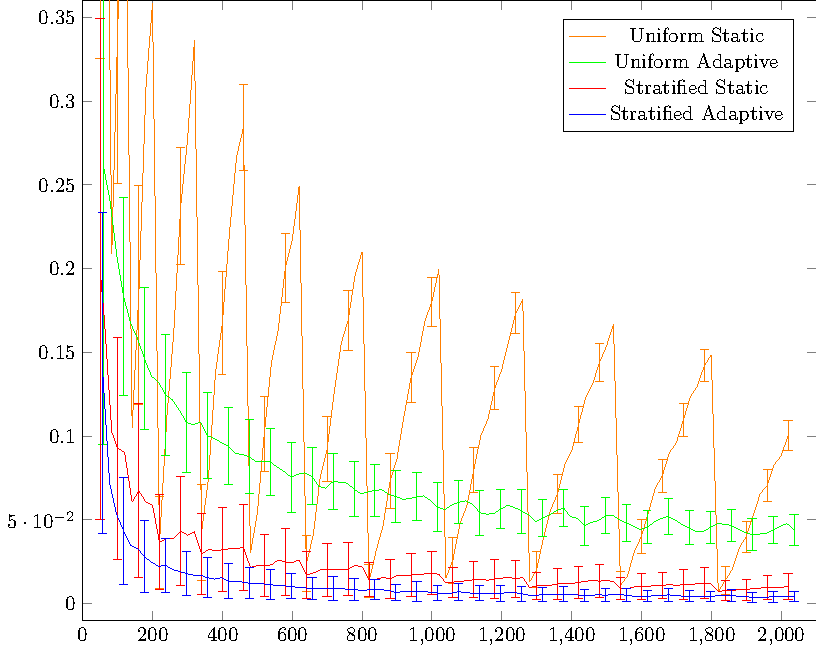
\includegraphics[scale=1 ]{graphs/graphtest.pdf}
  \caption{}
  \label{}
  \end{center}
\end{figure*}

INSERT RESULT TABLE
